\documentclass[conference]{IEEEtran}

\usepackage{cite}
\usepackage[utf8]{inputenc}
\usepackage[brazil]{babel}
\usepackage{amsmath,amssymb,amsfonts}
\usepackage{graphicx}
\usepackage{textcomp}
\usepackage{xcolor}
\usepackage{url}

\addto\captionsbrazil{\renewcommand{\abstractname}{Abstract}}

\def\BibTeX{{\rm B\kern-.05em{\sc i\kern-.025em b}\kern-.08em
    T\kern-.1667em\lower.7ex\hbox{E}\kern-.125emX}}

\sloppy

% Dados do trabalho
\newcommand{\tituloTrabalho}{Segmentação de Imagens Hiperespectrais Odontológicas\\ com Unmixing Espectral}
\newcommand{\autorTrabalho}{Ranulfo Mascari Neto}
\newcommand{\orientadorTrabalho}{Renato Ramos da Silva}
\newcommand{\instituicaoUm}{%
  Departamento de Ciência da Computação\\
  Universidade Federal de Lavras (UFLA)\\
  Lavras, MG, Brasil%
}
\newcommand{\instituicaoDois}{%
  Departamento de Computação Aplicada\\
  Universidade Federal de Lavras (UFLA)\\
  Lavras, MG, Brasil%
}
\newcommand{\emailAutor}{ranulfo.neto@estudante.ufla.br}
\newcommand{\emailOrientador}{renato.ramos@ufla.br}

\title{\tituloTrabalho}

\author{
\IEEEauthorblockN{\autorTrabalho}
\IEEEauthorblockA{\textit{Departamento de Ciência da Computação}\\
\textit{Universidade Federal de Lavras (UFLA)}\\
Lavras, MG, Brasil\\
\emailAutor}
\and
\IEEEauthorblockN{\orientadorTrabalho}
\IEEEauthorblockA{\textit{Departamento de Computação Aplicada}\\
\textit{Universidade Federal de Lavras (UFLA)}\\
Lavras, MG, Brasil\\
\emailOrientador}
}

\begin{document}

\maketitle

\begin{abstract}
  This work investigates semantic segmentation of oral and dental hyperspectral
  images using spectral unmixing as a physical-spectral guidance signal. The
  proposed approach preserves the original masks as the only semantic
  supervision and uses abundance maps inside attention gates of a dense U-Net.
  The model combines an AUnet backbone with an internal unmixing branch
  that learns abundance maps and a spectral reconstruction objective. The
  abundance maps modulate the skip connections, allowing the decoder to use both
  spatial context and spectral-mixture information. Experiments on the ODSI-DB
  are restricted to a controlled single-image protocol and compare Unet,
  AUnet, and the proposed Unmixing-Attention U-Net (UAUnet). Within this
  restricted protocol, the results indicate that attention gates improve
  sensitivity over Unet and that unmixing-guided gates provide additional gains
  under the same evaluation setting.
\end{abstract}

\section*{Resumo}
  Este trabalho investiga a segmentação semântica de imagens hiperespectrais
  orais e odontológicas usando \textit{unmixing} espectral como sinal de guia
  físico-espectral. A proposta preserva as máscaras originais como única
  supervisão semântica e usa mapas de abundância dentro dos \textit{attention
  gates} de uma U-Net densa. O modelo combina uma AUnet com um ramo interno de
  \textit{unmixing} que aprende mapas de abundância e uma reconstrução espectral
  auxiliar. Os mapas de abundância modulam as conexões de salto,
  permitindo que o decodificador utilize contexto espacial e informação de
  mistura espectral. Os experimentos no ODSI-DB são restritos a um protocolo
  controlado de imagem única e comparam Unet, AUnet e a
  Unmixing-Attention U-Net proposta (UAUnet). Sob esse protocolo restrito, os
  resultados indicam que os gates melhoram a sensibilidade em relação à Unet e
  que gates guiados por \textit{unmixing} fornecem ganhos adicionais na mesma
  configuração de avaliação.

\section{Introdução}

Imagens hiperespectrais têm sido investigadas em aplicações biomédicas por
combinarem informação espacial e espectral em uma única aquisição. Em
odontologia, essa característica é particularmente interessante porque tecidos e
estruturas orais podem apresentar respostas de reflectância distintas mesmo
quando suas diferenças visuais em RGB são sutis. O ODSI-DB foi proposto como
uma base pública de imagens espectrais orais e odontológicas, contendo imagens
de reflectância e anotações de especialistas para apoiar aplicações de visão
computacional em odontologia \cite{hyttinen2020odsi}.

Apesar desse potencial, a segmentação semântica em bases odontológicas
hiperespectrais permanece desafiadora. As máscaras disponíveis podem ser
esparsas, incompletas ou concentradas em regiões de maior confiança visual, e a
obtenção de anotações densas depende de conhecimento especializado. Esse cenário
é especialmente crítico quando o modelo supervisionado aprende apenas a partir de
pixels originalmente anotados, descartando regiões não anotadas que podem conter
informação espectral consistente com as classes de interesse.

Este trabalho parte da hipótese de que o \textit{unmixing} hiperespectral pode
fornecer um guia físico-espectral para a segmentação odontológica. As anotações
humanas são mantidas como única fonte de supervisão semântica, enquanto as
abundâncias estimadas pelo ramo de \textit{unmixing} são usadas para modular as
conexões de salto de uma AUnet. Desse modo, a fusão entre codificador
e decodificador é guiada por informação espectral interpretável, sem alterar o
alvo supervisionado da tarefa. Assim, a contribuição principal é uma arquitetura
de segmentação densa guiada por \textit{unmixing}, alinhada à natureza espacial
da segmentação odontológica.

\section{Trabalhos Relacionados}

O uso de imagens hiperespectrais em odontologia já foi explorado em trabalhos de
segmentação e análise automática. Boiko et al. \cite{boiko2019dentalhsi}
aplicaram redes profundas a imagens hiperespectrais odontológicas para segmentar
regiões e características clinicamente relevantes. Posteriormente, Garcia Peraza
Herrera et al. \cite{garcia2023odsisegmentation} avaliaram o ODSI-DB em
diferentes configurações de entrada, comparando imagens RGB, cubos
hiperespectrais e classificações baseadas apenas em pixels. Esses trabalhos
mostram que a informação espectral pode beneficiar a segmentação, mas concentram
a contribuição na entrada do segmentador. O presente trabalho usa a informação
espectral também dentro do próprio segmentador, por meio de \textit{attention
gates} guiados por mapas de abundância.

Como extensão arquitetural da U-Net, Oktay et al. \cite{oktay2018attentionunet}
propuseram a Attention U-Net, que incorpora \textit{attention gates} nas
conexões de salto entre codificador e decodificador. Esses mecanismos usam
informação contextual de escalas mais profundas para ponderar espacialmente as
características propagadas pelos \textit{skips}, reduzindo ativações em regiões
menos relevantes antes da concatenação no decodificador. Diferentemente de
abordagens de localização em múltiplos estágios, os autores integram os gates
diretamente à U-Net, mantendo uma arquitetura de segmentação densa treinável de
fim a fim. Essa ideia é particularmente pertinente em imagens médicas, nas quais
estruturas pequenas, bordas sutis e regiões de fundo podem dificultar a
recuperação de classes minoritárias.

No campo de \textit{unmixing} hiperespectral, Bioucas-Dias et al.
\cite{bioucasdias2012overview} apresentam uma visão ampla das abordagens
geométricas, estatísticas e baseadas em regressão esparsa. A NMF é uma das
formulações clássicas para esse problema, pois representa dados não negativos
como combinação de componentes também não negativos \cite{lee2000nmf}. Em
modelos neurais, Palsson et al. \cite{palsson2018autoencoder} mostram como
autoencoders podem ser estruturados para realizar \textit{blind unmixing},
interpretando a representação latente como abundâncias e o decodificador como
\textit{endmembers}. Uma comparação crítica posterior de autoencoders para
\textit{unmixing} reforça que escolhas arquiteturais e restrições físicas são
decisivas para a interpretabilidade do modelo \cite{palsson2022critical}.

Também há trabalhos recentes que conectam \textit{unmixing} e segmentação em
contextos biomédicos. Abdel Aziz et al. \cite{abdelaziz2025overlapped} defendem
o uso de mapas de abundância para representar tecidos sobrepostos, evitando a
limitação de máscaras binárias em pixels mistos. Essa perspectiva é adequada ao
ODSI-DB porque pixels de transição entre tecidos
podem carregar assinaturas espectrais mistas. O presente trabalho segue essa
linha ao usar abundâncias como um sinal contínuo e auxiliar dentro do
segmentador, sem convertê-las em rótulos discretos. A contribuição específica é
acoplar esse sinal aos \textit{attention gates} de uma U-Net, mantendo a saída
densa por pixel e a supervisão semântica original.

\section{Referencial Teórico}

Esta seção apresenta os fundamentos usados no trabalho: imagens
hiperespectrais, \textit{unmixing}, NMF, autoencoders, attention gates e
segmentação densa guiada por abundâncias.

\subsection{Imagens Hiperespectrais}

Uma imagem hiperespectral registra, para cada pixel, um vetor com medidas em
várias bandas do espectro eletromagnético. Diferentemente de uma imagem RGB, na
qual cada pixel é descrito por três canais, uma imagem hiperespectral forma um
cubo de dados com duas dimensões espaciais e uma dimensão espectral. Assim, um
pixel não é apenas uma cor, mas uma assinatura espectral que descreve como a
região observada responde em diferentes comprimentos de onda
\cite{bioucasdias2012overview}.

No contexto médico e biológico, essa representação é relevante porque a
interação da luz com tecidos depende de absorção, espalhamento, reflectância,
transmitância e fluorescência. Esses processos estão relacionados à composição e
à estrutura do tecido, incluindo a presença de cromóforos como hemoglobina,
melanina e água, além de alterações morfológicas e fisiológicas associadas a
diferentes condições clínicas \cite{lu2014medicalhsi}. Por isso, imagens
hiperespectrais podem revelar diferenças que não aparecem claramente em imagens
RGB, especialmente quando tecidos visualmente semelhantes apresentam respostas
espectrais distintas.

Neste projeto, essa propriedade é explorada no ODSI-DB, uma base pública de
imagens espectrais orais e odontológicas com anotações de especialistas
\cite{hyttinen2020odsi}. Cada pixel da cavidade oral é tratado como um espectro
de reflectância, e não apenas como uma intensidade RGB; por isso, a coerência
entre assinaturas espectrais é central para guiar a fusão entre informação
espacial e espectral no segmentador.

\subsection{Unmixing Hiperespectral}

Em imagens hiperespectrais, um pixel pode conter a contribuição de mais de um
material ou tecido. Isso ocorre por limitações de resolução espacial, por
misturas ópticas na superfície observada ou por transições entre regiões
anatômicas. O \textit{hyperspectral unmixing} busca decompor o espectro de cada
pixel em dois elementos: \textit{endmembers}, que representam assinaturas
espectrais de referência, e abundâncias, que indicam a contribuição de cada
\textit{endmember} no pixel \cite{bioucasdias2012overview}.

No modelo linear de mistura, a medição na banda espectral $i$ de um pixel pode
ser descrita por:

\[
y_i = \sum_{j=1}^{p} \rho_{ij}\alpha_j + w_i,
\]

em que $\rho_{ij}$ representa a resposta espectral do \textit{endmember} $j$ na
banda $i$, $\alpha_j$ é a abundância fracionária desse \textit{endmember},
$w_i$ representa ruído ou erro de modelagem, e $p$ é o número de
\textit{endmembers}. Em forma vetorial, a mesma relação pode ser escrita como:

\[
y = M\alpha + w,
\]

em que $M = [m_1, m_2, \ldots, m_p]$ é a matriz de mistura formada pelas
assinaturas espectrais dos \textit{endmembers}, $\alpha$ é o vetor de
abundâncias e $w$ representa a perturbação. Como as abundâncias representam
frações, elas geralmente são submetidas às restrições:

\[
\alpha_j \ge 0,\quad j = 1,\ldots,p,\qquad
\sum_{j=1}^{p}\alpha_j = 1.
\]

Ao organizar $Q$ pixels de uma imagem em uma matriz
$Y\in\mathbb{R}_{+}^{B\times Q}$, o modelo pode ser escrito de forma matricial
como $Y \approx MA$, em que $M\in\mathbb{R}_{+}^{B\times p}$ contém os
\textit{endmembers} e $A\in\mathbb{R}_{+}^{p\times Q}$ contém as abundâncias.
Para o projeto atual, essa decomposição tem duas funções. Primeiro, ela permite
aprender assinaturas espectrais representativas das estruturas odontológicas
presentes em uma imagem. Segundo, os mapas de abundância fornecem uma medida
contínua de associação entre cada pixel e cada componente espectral, o que é
usado posteriormente para guiar os \textit{attention gates} sem modificar os
rótulos supervisionados.

\subsection{Fatoração de Matrizes Não Negativas}

A fatoração de matrizes não negativas, ou \textit{Non-negative Matrix
Factorization} (NMF), é uma técnica de decomposição que aproxima uma matriz de
dados não negativa pelo produto de duas matrizes também não negativas. Dada uma
matriz de dados $V$, a NMF busca uma reconstrução $\hat{V}$ dada por:

\[
\hat{V} = HW,
\]

em que $H$ representa os componentes de base e $W$ representa os pesos de cada
componente na reconstrução das observações. Essa formulação é baseada na
restrição de não negatividade, que favorece representações aditivas dos dados
\cite{lee2000nmf}. Quando aplicada ao \textit{unmixing} hiperespectral, essa
decomposição possui uma interpretação natural: os componentes de $H$ podem ser
associados aos \textit{endmembers}, enquanto os valores de $W$ podem ser
interpretados como abundâncias desses componentes em cada pixel. Essa relação é
particularmente adequada para imagens de
reflectância, pois os dados observados, as assinaturas espectrais e as
abundâncias possuem interpretação não negativa.

No projeto, a NMF não é usada como modelo final isolado. Ainda assim, ela fornece
a base conceitual para interpretar o \textit{unmixing} como uma decomposição de
espectros em componentes e pesos. Essa interpretação é importante porque o
autoencoder adotado também reconstrói a imagem a partir de uma representação
latente não negativa: a camada latente representa abundâncias, enquanto o
decodificador representa os \textit{endmembers}.

Uma variação relevante para relacionar NMF e redes neurais é a NMF convexa. Nessa
formulação, os componentes de base são restringidos a combinações das próprias
observações da matriz de dados. A reconstrução passa a ser escrita como
\cite{egendal2024relation}:

\[
\hat{V} = V W_1 W_2.
\]

Definindo $H := V W_1$ e $W := W_2$, essa expressão preserva a forma geral da
NMF, isto é, $\hat{V} = HW$. A diferença é que, na NMF convexa, a matriz de base
$H$ não é estimada livremente: ela é obtida a partir da própria matriz $V$.

\subsection{Autoencoders}

Autoencoders são modelos neurais treinados para reconstruir sua própria entrada.
Eles possuem uma etapa de codificação, que transforma o dado de entrada em uma
representação latente, e uma etapa de decodificação, que reconstrói o dado
original a partir dessa representação. Quando a dimensão latente é menor que a
dimensão de entrada, o modelo aprende uma representação compacta dos dados.

No contexto de \textit{unmixing} hiperespectral, Palsson et al.
\cite{palsson2018autoencoder} formulam o uso de autoencoders a partir do modelo
linear de mistura. Para um pixel $x_p$, o modelo assume:

\[
x_p = M s_p + n_p,
\]

em que $M$ é a matriz de \textit{endmembers}, $s_p$ é o vetor de abundâncias do
pixel e $n_p$ representa ruído. Considerando todos os pixels da imagem, essa
relação pode ser escrita como:

\[
X = MS + N.
\]

Essa formulação impõe uma interpretação direta à arquitetura do autoencoder. O
codificador $G_E$ mapeia o espectro de entrada $x_p$ para uma representação
latente $h_p$, enquanto o decodificador $G_D$ reconstrói o espectro a partir
dessa representação:

\[
\hat{x}_p = G_D(G_E(x_p)).
\]

Como a reconstrução final deve obedecer ao modelo linear de mistura, o
decodificador é restringido a uma transformação linear. Assim, a última camada
latente deve ter dimensão igual ao número de \textit{endmembers}; suas ativações
são interpretadas como as abundâncias $s_p$, e os pesos do decodificador são
interpretados como as colunas da matriz $M$, isto é, os espectros dos
\textit{endmembers}. Dessa forma, após o treinamento, o autoencoder realiza
\textit{blind unmixing}: estima simultaneamente mapas de abundância e assinaturas
espectrais a partir da própria imagem.

Essa interpretação exige restrições compatíveis com o modelo físico de mistura.
Em particular, as abundâncias devem satisfazer a restrição de não negatividade e,
frequentemente, a restrição de soma unitária. O modelo adotado segue essa
ideia por meio de um ramo interno de \textit{unmixing}: o codificador estima
mapas de abundância não negativos, a normalização por soma impõe uma
interpretação fracionária por pixel, e o decodificador espectral reconstrói os
espectros de reflectância a partir de \textit{endmembers} latentes. Assim, a
saída auxiliar do modelo não é apenas uma reconstrução, mas também um conjunto
interpretável de mapas de abundância e \textit{endmembers}.

Palsson et al. \cite{palsson2018autoencoder} destacam ainda que a função
objetivo deve preservar a forma espectral. Por isso, o projeto utiliza a
distância angular espectral (\textit{Spectral Angle Distance} -- SAD) como perda
de reconstrução. Para um espectro observado $x$ e sua reconstrução $\hat{x}$, a
SAD é dada por:

\[
\mathrm{SAD}(x,\hat{x}) =
\arccos\left(\frac{x^{T}\hat{x}}{\|x\|_2\|\hat{x}\|_2}\right).
\]

Essa medida compara a direção dos vetores espectrais, reduzindo a dependência de
diferenças de escala e enfatizando a similaridade da assinatura espectral. No
projeto, a SAD é usada como termo auxiliar de reconstrução no treinamento
conjunto da U-Net guiada por \textit{unmixing}, incentivando que as abundâncias
usadas pelos gates mantenham coerência físico-espectral.

De forma complementar, a relação entre autoencoders não negativos e NMF fornece
uma base teórica para essa interpretação. Quando um autoencoder é raso, linear,
sem termos de viés, com ativações identidade e pesos não negativos, sua
reconstrução pode ser escrita como:

\[
\hat{V} = V W_{\mathrm{enc}} W_{\mathrm{dec}}.
\]

Essa expressão tem a mesma forma da NMF convexa, com
$W_1 = W_{\mathrm{enc}}$ e $W_2 = W_{\mathrm{dec}}$
\cite{egendal2024relation}. Portanto, enquanto o trabalho de Palsson et al.
fundamenta o uso de autoencoders para \textit{unmixing} hiperespectral, essa
equivalência ajuda a entender por que autoencoders não negativos podem ser
interpretados como modelos próximos a fatorações matriciais. Essa interpretação,
porém, depende das restrições impostas ao modelo: arquiteturas mais profundas,
ativações não lineares ou outras estratégias de não negatividade aumentam a
flexibilidade, mas reduzem a equivalência direta com a NMF.

\subsection{Segmentação Semântica Hiperespectral}

Segmentação semântica é a tarefa de atribuir uma classe a cada pixel da imagem.
Em imagens hiperespectrais, essa tarefa pode explorar tanto a organização
espacial da cena quanto a assinatura espectral de cada pixel. No ODSI-DB, as
classes correspondem a regiões e estruturas odontológicas anotadas por
especialistas, o que torna a segmentação dependente de informação local,
contexto espacial e diferenças espectrais sutis entre tecidos.

O projeto utiliza uma arquitetura do tipo U-Net como segmentador supervisionado.
A U-Net foi proposta para segmentação biomédica e combina uma trilha de
contração, que extrai contexto, com uma trilha de expansão, que recupera
resolução espacial, usando conexões entre níveis correspondentes da rede
\cite{ronneberger2015unet}. Aqui, essa arquitetura é aplicada diretamente aos
cubos hiperespectrais odontológicos.

Essa etapa estabelece a tarefa final do trabalho: produzir máscaras semânticas a
partir de imagens hiperespectrais odontológicas. O modelo espectral atua em
paralelo ao segmentador, como guia contínuo para os \textit{attention gates}.

\subsection{Attention Gates em U-Net}

A U-Net original reutiliza mapas de características do codificador por meio de
conexões de salto. Essas conexões ajudam a recuperar detalhes espaciais perdidos
nas etapas de subamostragem, mas propagam todos os padrões extraídos pelo
codificador, inclusive respostas de fundo ou regiões pouco informativas. A
Attention U-Net modifica esse ponto específico da arquitetura: antes da
concatenação com o decodificador, cada \textit{skip} é multiplicado por um mapa
de atenção espacial aprendido \cite{oktay2018attentionunet}.

Seja $x_l$ o mapa de características vindo do codificador no nível $l$ e $g_l$
o sinal de contexto vindo do decodificador em escala compatível. O gate calcula
coeficientes espaciais $\alpha_l \in [0,1]$ a partir de uma forma aditiva de
atenção:

\[
\alpha_l =
\sigma\left(
\psi^{T}
\mathrm{ReLU}\left(W_x x_l + W_g g_l + b\right)
\right),
\]

em que $W_x$, $W_g$ e $\psi$ são projeções aprendidas, $b$ representa termos de
viés e $\sigma$ é a função sigmoide. O mapa propagado pelo \textit{skip} passa a
ser:

\[
\hat{x}_l = \alpha_l \odot x_l.
\]

Desse modo, regiões consideradas relevantes pelo contexto do decodificador são
preservadas, enquanto regiões menos informativas têm sua contribuição reduzida.
No trabalho de Oktay et al. \cite{oktay2018attentionunet}, essa operação é
introduzida para aumentar a sensibilidade em estruturas anatômicas difíceis,
sem exigir um detector de região de interesse separado. No presente trabalho, a
mesma ideia é usada como uma ablação arquitetural: avaliar se filtrar as
conexões de salto da U-Net hiperespectral melhora a segmentação no ODSI-DB
antes de introduzir mecanismos espectrais adicionais.

\subsection{Segmentação Guiada por Unmixing}

Em uma imagem hiperespectral, o vetor espectral de um pixel pode ser interpretado
como mistura de componentes latentes associados a materiais ou tecidos. Para
segmentação semântica, essa interpretação pode ser usada como sinal auxiliar
interno ao modelo. Neste trabalho, os mapas de abundância são mantidos como
variáveis contínuas e usados para regular a fusão de características espaciais
na U-Net. Assim, o \textit{unmixing} atua como guia físico-espectral da
arquitetura, enquanto a anotação humana continua definindo a supervisão
semântica.

A abordagem proposta combina essa interpretação espectral com a natureza densa
da segmentação. As abundâncias não definem a classe final do pixel; elas
influenciam apenas a passagem de características nas conexões de salto. Dessa
forma, a decisão semântica continua sendo feita pela U-Net, enquanto o
\textit{unmixing} fornece um indício físico-espectral sobre quais regiões do
codificador devem ser preservadas com maior intensidade pelo decodificador.

\section{Metodologia}

\subsection{Base de Dados e Pré-processamento}

Os experimentos utilizam cubos de reflectância do ODSI-DB interpolados para
$B=170$ bandas igualmente espaçadas entre 450 nm e 950 nm. Seja

\[
\mathcal{D}=\{(X_i,Y_i)\}_{i=1}^{N}
\]

o conjunto de imagens anotadas, em que
$X_i\in\mathbb{R}_{+}^{B\times H_i\times W_i}$ representa o cubo de
reflectância da imagem $i$ e
$Y_i\in\{0,1\}^{C\times H_i\times W_i}$ representa a máscara multiclasse, com
$C=35$ classes odontológicas. Como as anotações do ODSI-DB não são
necessariamente densas, define-se o conjunto de pixels originalmente rotulados
por:

\[
\Omega_i^{L} =
\left\{p \in \Omega_i :
\sum_{c=1}^{C}Y_{i,c,p}=1
\right\},
\]

em que $\Omega_i$ é o domínio espacial da imagem $i$. Pixels fora de
$\Omega_i^{L}$ não contribuem para a perda supervisionada da linha de base.

Para o treinamento do segmentador, a entrada interpolada é normalizada por
vetores de média e desvio padrão pré-computados para cada banda. Na UAUnet, o
mesmo cubo também alimenta o ramo de \textit{unmixing}, cuja reconstrução é
comparada contra a reflectância. A avaliação é feita apenas nos pixels anotados
reservados para teste no protocolo de imagem única; portanto, esse protocolo
mede uma comparação controlada dentro de uma cena, e não generalização entre
pacientes ou entre imagens.

\subsection{Ramo de Unmixing da UAUnet}

A UAUnet reportada recebe a imagem hiperespectral normalizada
$X_i\in\mathbb{R}^{B\times H_i\times W_i}$ e estima internamente um conjunto de
$P=48$ mapas de abundância. O objetivo desse ramo não é classificar pixels, mas
produzir um sinal físico-espectral auxiliar que possa guiar os
\textit{attention gates}. Primeiro, uma convolução $3\times3$ projeta as
$B=170$ bandas para $D=64$ canais, seguida de normalização em lote e GELU:

\[
F_i = \phi_{\mathrm{emb}}(X_i).
\]

Em seguida, um bloco leve de atenção no eixo dos canais e um codificador
baseado em convoluções $1\times1$ estimam os logits de abundância, com
dimensões $64\rightarrow32\rightarrow16\rightarrow P$. Se $z_{p,q}$ é o logit
do componente latente $p$ no pixel $q$, as abundâncias são normalizadas para
respeitar não negatividade e soma unitária:

\[
a_{p,q} =
\frac{|z_{p,q}|}
{\max\left(\sum_{s=1}^{P}|z_{s,q}|,\epsilon\right)}.
\]

\[
a_{p,q}\ge 0,\qquad
\sum_{p=1}^{P}a_{p,q}\approx 1.
\]

A reconstrução espectral auxiliar usa $R=10$ variantes por \textit{endmember}.
Se $e_{p,r}\in\mathbb{R}^{B}$ é a variante $r$ do componente $p$ e
$\gamma_{p,r,q}$ é o peso obtido por \textit{softmax} entre variantes no pixel
$q$, então a reconstrução do espectro desse pixel pode ser escrita como:

\[
\hat{x}_q =
\sum_{p=1}^{P} a_{p,q}
\sum_{r=1}^{R}\gamma_{p,r,q}e_{p,r}.
\]

Essa reconstrução força o ramo de \textit{unmixing} a manter relação com os
espectros de reflectância observados, em vez de se tornar apenas uma
representação discriminativa livre. Nenhum componente latente é mapeado
diretamente para uma classe odontológica; as abundâncias permanecem como
variáveis contínuas que guiam a segmentação.

\subsection{U-Net Guiada por Abundâncias}

A trilha principal de segmentação é uma AUnet com a mesma estrutura
básica da U-Net de referência: três blocos descendentes, três blocos ascendentes
e duas conexões de salto usadas pelo decodificador. A diferença da versão guiada
está no cálculo dos mapas de atenção dos \textit{skips}. Para cada conexão de
salto, calcula-se primeiro um gate puramente espacial, dependente do mapa do
codificador $x_l$ e do sinal do decodificador $g_l$:

\[
\alpha_l^{\mathrm{base}} =
\sigma\left(
\psi^{T}
\mathrm{ReLU}(W_xx_l+W_gg_l+b)
\right).
\]

Em paralelo, calcula-se um gate guiado por abundâncias, no qual o mapa de
abundâncias $A_i$ é redimensionado para a escala do \textit{skip} e projetado
para o mesmo espaço intermediário:

\[
\alpha_l^{\mathrm{guiado}} =
\sigma\left(
\psi^{T}
\mathrm{ReLU}(W_xx_l+W_gg_l+W_aA_i+b)
\right).
\]

Para manter a ablação próxima da AUnet e evitar que o guia espectral
domine a segmentação no início do treinamento, os dois mapas são combinados de
forma residual:

\[
\alpha_l =
(1-\eta)\alpha_l^{\mathrm{base}} +
\eta\alpha_l^{\mathrm{guiado}},
\qquad \eta=0{,}10.
\]

O \textit{skip} final é $\hat{x}_l=\alpha_l\odot x_l$. Nos experimentos, as
abundâncias usadas pelos gates são destacadas do gradiente da perda semântica.
Assim, a segmentação aprende com as máscaras humanas originais, enquanto o ramo
de \textit{unmixing} é orientado pela reconstrução espectral. Essa escolha
preserva o caráter físico das abundâncias e reduz o risco de que elas se tornem
apenas variáveis latentes discriminativas sem interpretação espectral.

\subsection{Treinamento e Avaliação da Segmentação}

A segmentação é realizada com modelos que recebem $B=170$ canais de entrada e
produzem 35 mapas de classe. A comparação metodológica deste artigo é restrita
ao protocolo controlado de imagem única. A mesma imagem clínica é usada em
todos os experimentos; para cada classe
anotada, 1\% dos pixels é reservado para treino, 1\% para validação e o restante
para teste. Essa escolha permite comparar os modelos sob o mesmo cubo
hiperespectral, a mesma distribuição de pixels anotados e a mesma supervisão
humana original.

Três modelos são avaliados. O primeiro é a Unet, uma U-Net densa usada
como linha de base. O segundo é a AUnet, que preserva a estrutura da
Unet, mas insere \textit{attention gates} nas conexões de salto. O terceiro
é a UAUnet, que mantém a mesma trilha U-Net com gates, mas adiciona o ramo de
\textit{unmixing} com variantes de \textit{endmembers} descrito anteriormente
para estimar abundâncias e usá-las como guia físico-espectral dos gates. Assim,
a comparação isola duas perguntas: o efeito dos gates em relação à Unet e o
efeito adicional do guia por abundâncias em relação à AUnet.

Como nem todos os pixels possuem anotação, a perda de segmentação é calculada
apenas no conjunto de pixels rotulados da máscara humana original. Define-se:

\[
\Omega_i^{L}=
\left\{p\in\Omega_i:\sum_{c=1}^{C}Y_{i,c,p}=1\right\}.
\]

A função objetivo supervisionada por imagem é a entropia cruzada negativa
ponderada por classe:

\[
\ell_i =
\frac{
\sum_{p \in \Omega_i^{L}}
w_{y_p}\left[-\log P(y_p|x_p)\right]
}{
\sum_{p \in \Omega_i^{L}} w_{y_p}
}.
\]
em que $w_{y_p}$ é o peso da classe, $y_p$ é o rótulo do pixel e $P(y_p|x_p)$ é
a probabilidade prevista para a classe correta. No treinamento, a perda do lote
é:

\[
\mathcal{L}_{\mathrm{seg}} =
\frac{1}{|\mathcal{B}^{+}|}
\sum_{i\in\mathcal{B}^{+}}\ell_i,
\]

em que $\mathcal{B}^{+}$ é o subconjunto de imagens do lote que possuem ao
menos um pixel anotado.

Unet e AUnet são treinadas apenas com
$\mathcal{L}_{\mathrm{seg}}$. Na UAUnet, a perda total combina a perda semântica
com termos físico-espectrais associados ao ramo de \textit{unmixing}:

\[
\mathcal{L} =
\mathcal{L}_{\mathrm{seg}}
+ \lambda_{\mathrm{sad}}\mathcal{L}_{\mathrm{SAD}}
+ \lambda_{1/2}\mathcal{L}_{1/2}
+ \lambda_{\mathrm{div}}\mathcal{L}_{\mathrm{div}}.
\]

O termo $\mathcal{L}_{\mathrm{SAD}}$ é a distância angular espectral entre
$X_i$ e $\hat{X}_i$, $\mathcal{L}_{1/2}$ é uma penalização de esparsidade
$L_{1/2}$ sobre as abundâncias, e $\mathcal{L}_{\mathrm{div}}$ penaliza
similaridade excessiva entre \textit{endmembers}. Nos experimentos com UAUnet,
foram usados $\lambda_{\mathrm{sad}}=0{,}01$,
$\lambda_{1/2}=0{,}001$ e $\lambda_{\mathrm{div}}=0{,}001$. Em todos os casos,
a saída de segmentação é avaliada no mesmo conjunto de pixels de teste.

A avaliação é feita no conjunto de teste usando acurácia, sensibilidade,
especificidade e acurácia balanceada. Para cada classe, as probabilidades
previstas são binarizadas com limiar 0,5 nos pixels anotados, e as métricas são
definidas por:

\[
\mathrm{Acc}=\frac{TP+TN}{TP+TN+FP+FN},\qquad
\mathrm{Sens}=\frac{TP}{TP+FN},
\]

\[
\mathrm{Spec}=\frac{TN}{TN+FP},\qquad
\mathrm{BAcc}=\frac{\mathrm{Sens}+\mathrm{Spec}}{2}.
\]

Os valores globais reportados nos resultados são médias por classe sobre as
classes do conjunto de interesse que possuem pixels positivos no teste. Na
imagem usada, esse subconjunto é formado por pele, mucosa oral, esmalte,
gengiva inserida e cabelo. Classes ausentes no teste não entram nessas médias,
para evitar que acurácia e especificidade sejam artificialmente infladas por
verdadeiros negativos triviais.

\section{Resultados e Discussão}

Os resultados da Tabela~\ref{tab:single-image-results} comparam Unet,
AUnet e UAUnet no mesmo protocolo de imagem única. Todos os modelos usam a
mesma imagem clínica, a mesma divisão 1\%/1\%/98\% dos pixels
anotados por classe e as mesmas máscaras humanas originais. Assim, as diferenças
observadas são compatíveis com as mudanças arquiteturais avaliadas: inclusão de
\textit{attention gates} e, em seguida, uso de abundâncias como guia desses
gates.

\begin{table}[ht]
\centering
\caption{Comparação no protocolo de imagem única.}
\label{tab:single-image-results}
\begin{tabular}{lrrrr}
\hline
Modelo & Acc. & BAcc. & Sens. & Spec. \\
\hline
Unet & 0,956 & 0,825 & 0,654 & 0,997 \\
AUnet & 0,958 & 0,851 & 0,703 & 0,998 \\
UAUnet & 0,964 & 0,884 & 0,771 & 0,998 \\
\hline
\end{tabular}
\end{table}

A Figura~\ref{fig:prediction-visualizations} apresenta visualizações
qualitativas das predições na mesma imagem usada no protocolo experimental.
Essas visualizações não substituem as métricas da Tabela~\ref{tab:single-image-results},
mas permitem inspecionar a distribuição espacial dos erros e acertos dos três
modelos.

\begin{figure*}[t]
\centering
\begin{tabular}{@{}ccccc@{}}
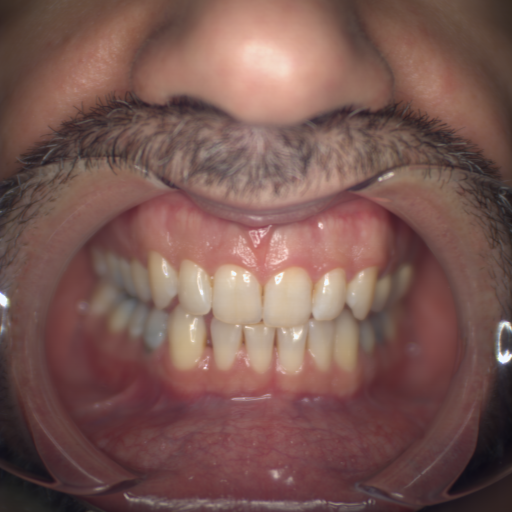
\includegraphics[width=0.18\textwidth]{figures/pred_input_rgb.png} &
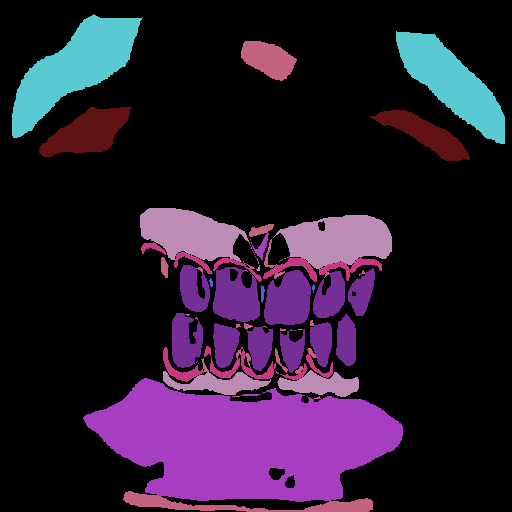
\includegraphics[width=0.18\textwidth]{figures/pred_ground_truth.png} &
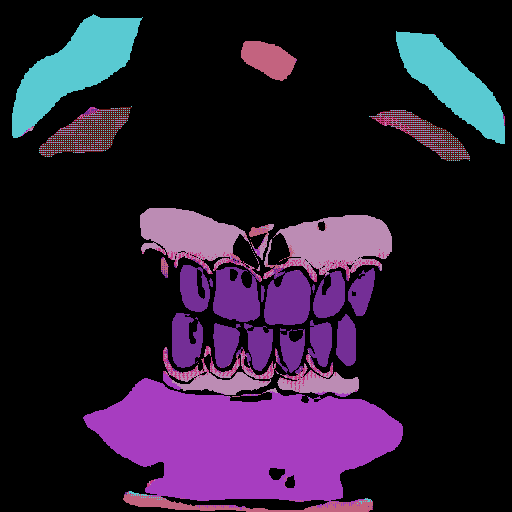
\includegraphics[width=0.18\textwidth]{figures/pred_unet_annotated.png} &
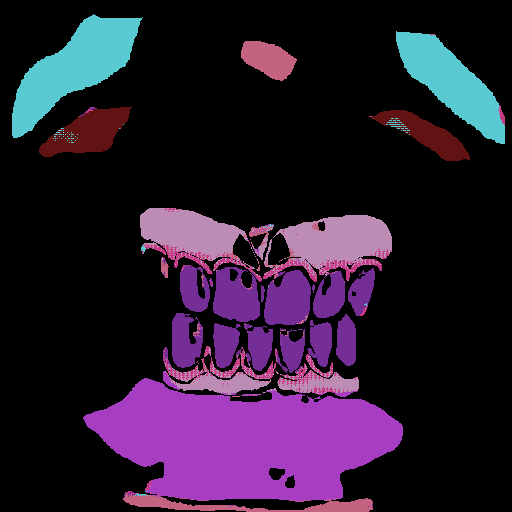
\includegraphics[width=0.18\textwidth]{figures/pred_aunet_annotated.png} &
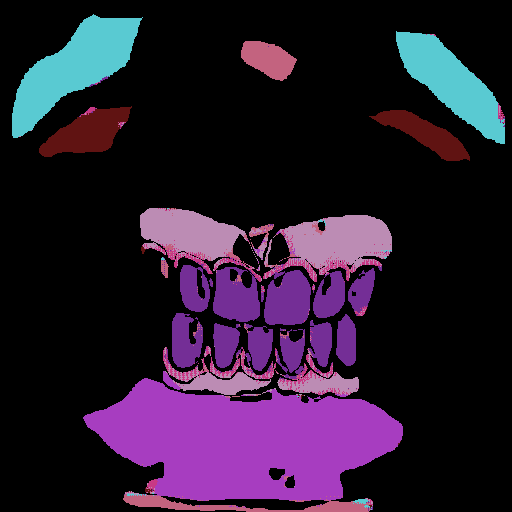
\includegraphics[width=0.18\textwidth]{figures/pred_uau_annotated.png} \\
\scriptsize Entrada RGB & \scriptsize Máscara & \scriptsize Pred. Unet &
\scriptsize Pred. AUnet & \scriptsize Pred. UAUnet \\[0.5em]
\end{tabular}
\begin{tabular}{@{}ccc@{}}
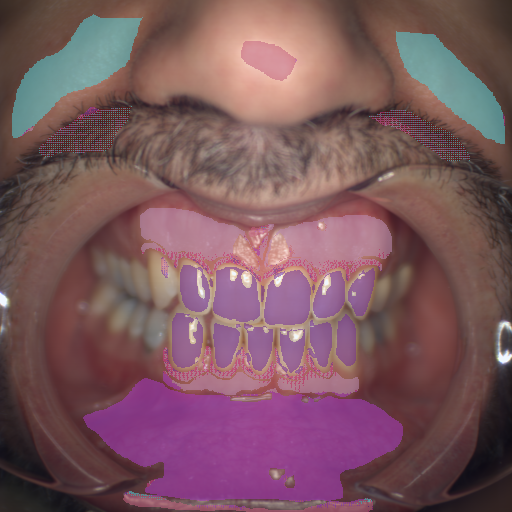
\includegraphics[width=0.31\textwidth]{figures/overlay_unet_annotated.png} &
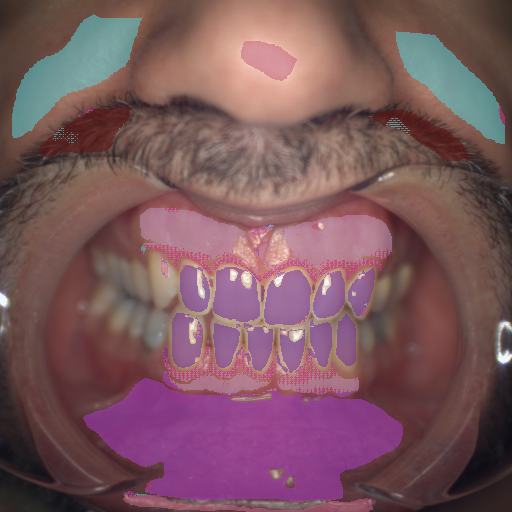
\includegraphics[width=0.31\textwidth]{figures/overlay_aunet_annotated.png} &
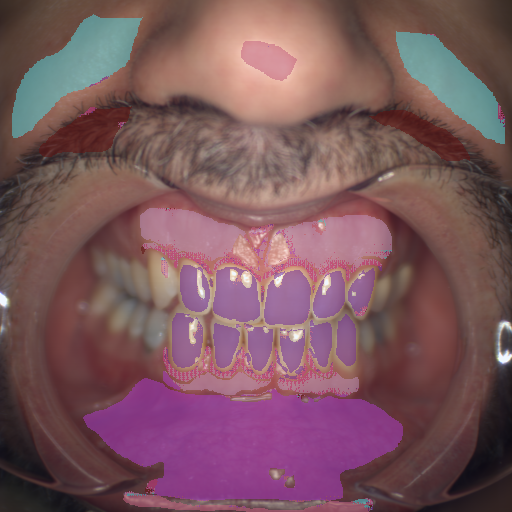
\includegraphics[width=0.31\textwidth]{figures/overlay_uau_annotated.png} \\
\scriptsize Sobreposição Unet & \scriptsize Sobreposição AUnet &
\scriptsize Sobreposição UAUnet
\end{tabular}
\caption{Visualização qualitativa das predições no protocolo de imagem única.
O painel superior mostra a imagem RGB, a máscara humana anotada e as predições
dos três modelos restritas aos pixels anotados. O painel inferior mostra as
mesmas predições sobrepostas à imagem RGB. Todas as visualizações usam a mesma
imagem clínica e as mesmas máscaras humanas originais.}
\label{fig:prediction-visualizations}
\end{figure*}

AUnet melhora a acurácia balanceada de 0,825 para 0,851 e a
sensibilidade de 0,654 para 0,703 em relação à Unet. Esse resultado é
coerente com a proposta da Attention U-Net \cite{oktay2018attentionunet}: os
gates atuam nas conexões de salto e reduzem a propagação de ativações menos
relevantes, favorecendo a recuperação de pixels positivos em classes de
interesse. A acurácia e a especificidade permanecem muito altas nos dois
modelos, o que indica que a principal diferença aparece na capacidade de
recuperar regiões anotadas, e não na rejeição de pixels negativos.

A UAUnet apresenta o melhor desempenho entre os três modelos, com acurácia
balanceada de 0,884 e sensibilidade de 0,771. Em relação à AUnet, o
ganho é de 0,034 em acurácia balanceada e 0,068 em sensibilidade. Em relação à
Unet, o ganho acumulado é de 0,059 em acurácia balanceada e 0,117 em
sensibilidade. Como a especificidade se mantém próxima de 0,998, o aumento de
sensibilidade não ocorre à custa de uma queda expressiva na identificação de
pixels negativos.

Esses resultados são compatíveis com a hipótese central do trabalho:
abundâncias de \textit{unmixing} podem ser úteis como guia contínuo dos
\textit{attention gates}. A Unet fornece a linha de base densa; a AUnet
mostra o efeito de filtrar espacialmente os \textit{skips}; e a UAUnet adiciona
um critério físico-espectral a essa filtragem. Portanto, a melhoria da UAUnet
neste ensaio sugere que a informação espectral da mistura de tecidos ajuda a
decidir quais características do codificador devem ser preservadas pelo
decodificador durante a segmentação.

A principal limitação metodológica é que o protocolo é restrito a uma única
imagem. A divisão por pixels permite uma comparação controlada entre
arquiteturas, mas não mede robustez entre pacientes, variação entre câmeras ou
generalização para outras cenas do ODSI-DB. Assim, os resultados devem ser
interpretados como uma evidência inicial de ablação, não como validação clínica
ou estatística ampla da arquitetura.

\section{Conclusão}

Este trabalho apresentou uma abordagem para segmentação de imagens
hiperespectrais odontológicas no ODSI-DB usando \textit{unmixing} espectral como
guia interno de uma U-Net densa. A proposta preserva as máscaras humanas como
única supervisão semântica e usa abundâncias e reconstrução espectral para
modular os \textit{attention gates} das conexões de salto.

No protocolo de imagem única, a comparação entre Unet, AUnet e UAUnet
mostrou ganhos progressivos em acurácia balanceada e sensibilidade. AUnet
melhorou a recuperação de pixels positivos em relação à Unet,
e a UAUnet obteve o melhor resultado ao adicionar o guia físico-espectral de
\textit{unmixing} aos gates. A principal evidência metodológica é que, nesse
ensaio controlado, abundâncias podem ser úteis como sinal contínuo de guia
físico-espectral. Como trabalhos futuros, destacam-se a avaliação em múltiplas
imagens e sujeitos, a análise quantitativa dos mapas de abundância, a inspeção
dos mapas de gate e a investigação de formas adicionais de tornar o guia
espectral mais interpretável.

\clearpage

\bibliographystyle{ieeetr}
\bibliography{sbc-template}

\end{document}
